\chapter{Discussion}
	This chapter will summarise and discuss the results given in the previous chapter.

\section{Guidance System}
	This guidance system are designed for long, straight pipeline stretches. It will not be able to handle
	sudden turns in the pipeline direction, without specifying this in the guidance system. This can be
	included as waypoints where the pipeline are changing, and be included as a condition; \textit{when the AUV
	reaches certain position the direction of the pipeline changes}. This requires very exact knowledge
	about the pipeline and are really the case. This is why there should be a more autonomous way of
	doing this. This motivates the use of more sensors than just a camera to follow the pipeline. The
	camera have a very limited field of view, usually restricted to less than 3 meters. A Sidescan Sonar
	combined with a Forward Looking Sonar, which provides sensor data of the pipeline in front of the AUV
	will give the guidance system some data to decide and predict what it will do if there is a sharp
	turn in the pipeline.

	Sharp turns are a product of T-junctions and other couplings of pipelines. These
	junctions are usually well documented, and given good and exact locations. But if the navigation
	sensors of the AUV have large uncertainties, it might look as they are in the wrong
	place, for the AUV. This suggests that information about the pipeline should be treated with care. Because the
	errors in an AUV navigation system might be substantial and provide that \'a priori information about
	the pipeline will be unusable. 

	The navigation system of \textit{HUGIN 1000} are a Velocity Aided Inertial Navigation System. This
	utilises a Doppler Velocity Log to measure the velocity relatively to the sea bottom and input this to
	the INS system. The INS systems installed on the \hugin are in the 1 nmi/h class, i.e the INS system drifts
 	less than 1 nmi in an hour. This results in a drift in the navigation system equal to
	0.11 \% of the travelled distance along the track, and about 0.03 \% error in the across distance of a
	straight line track according to \cite{INS_Hugin}. This can be enough to throw the guidance system off
	course, because the field of view of the camera are relatively small.

	There are ways of improving the INS drift and thereby improving the position estimate, one is to use 
	GPS update fixes, but this requires to
	surface the AUV once in a while. This is of course not a good idea when the AUV are at great depths.
	There are possibilities to use sea bottom anchored position buoys, which exact position are known and
	the AUV might use these buoys by pinging them and getting a updated position estimate. This is a good
	idea if the pipeline infrastructure admits this. Say that this position buoys are placed at the same
	time as the pipeline are laid.

	The problem regarding when $\psi \rightarrow 2\pi$, as mentioned in the previous chapter is a
	implementation issue. There are a number of solutions for this.
	The first is to limit the sensor output, which is the case in the real world, since a compass
	measuring \textit{yaw} only are defined for $(0, 2 \pi)$. The controller can handle this by including
	a check whether if its heading are larger than $\pi$, the given command will be to the right, and
	opposite if the measured heading are smaller than $\pi$.



\section{Roll Stabilisation}
	The mission of the AUV are to provide good data for later use, i.e good pictures to be analysed later.
	The camera on the AUV are mounted downwards and the field of view are affected by roll and pitch.
	Pitch are a control angle, but the Roll motion have no direct control measures. The roll angle need to
	be as close to 0 as possible to provide best pictures of the current sea bottom.
	The plots in Figure~\ref{fig:ch4_rollyawmoment}
	are taken from the $4^{\mathrm{th}}$ Scenario described in Chapter~\ref{ch3}, to look at \hugin's 
	stability in roll.

	\begin{figure}[htbp]
		\centering
		\subfigure[Roll Angle]{
			\label{fig:ch4_rollangle}
			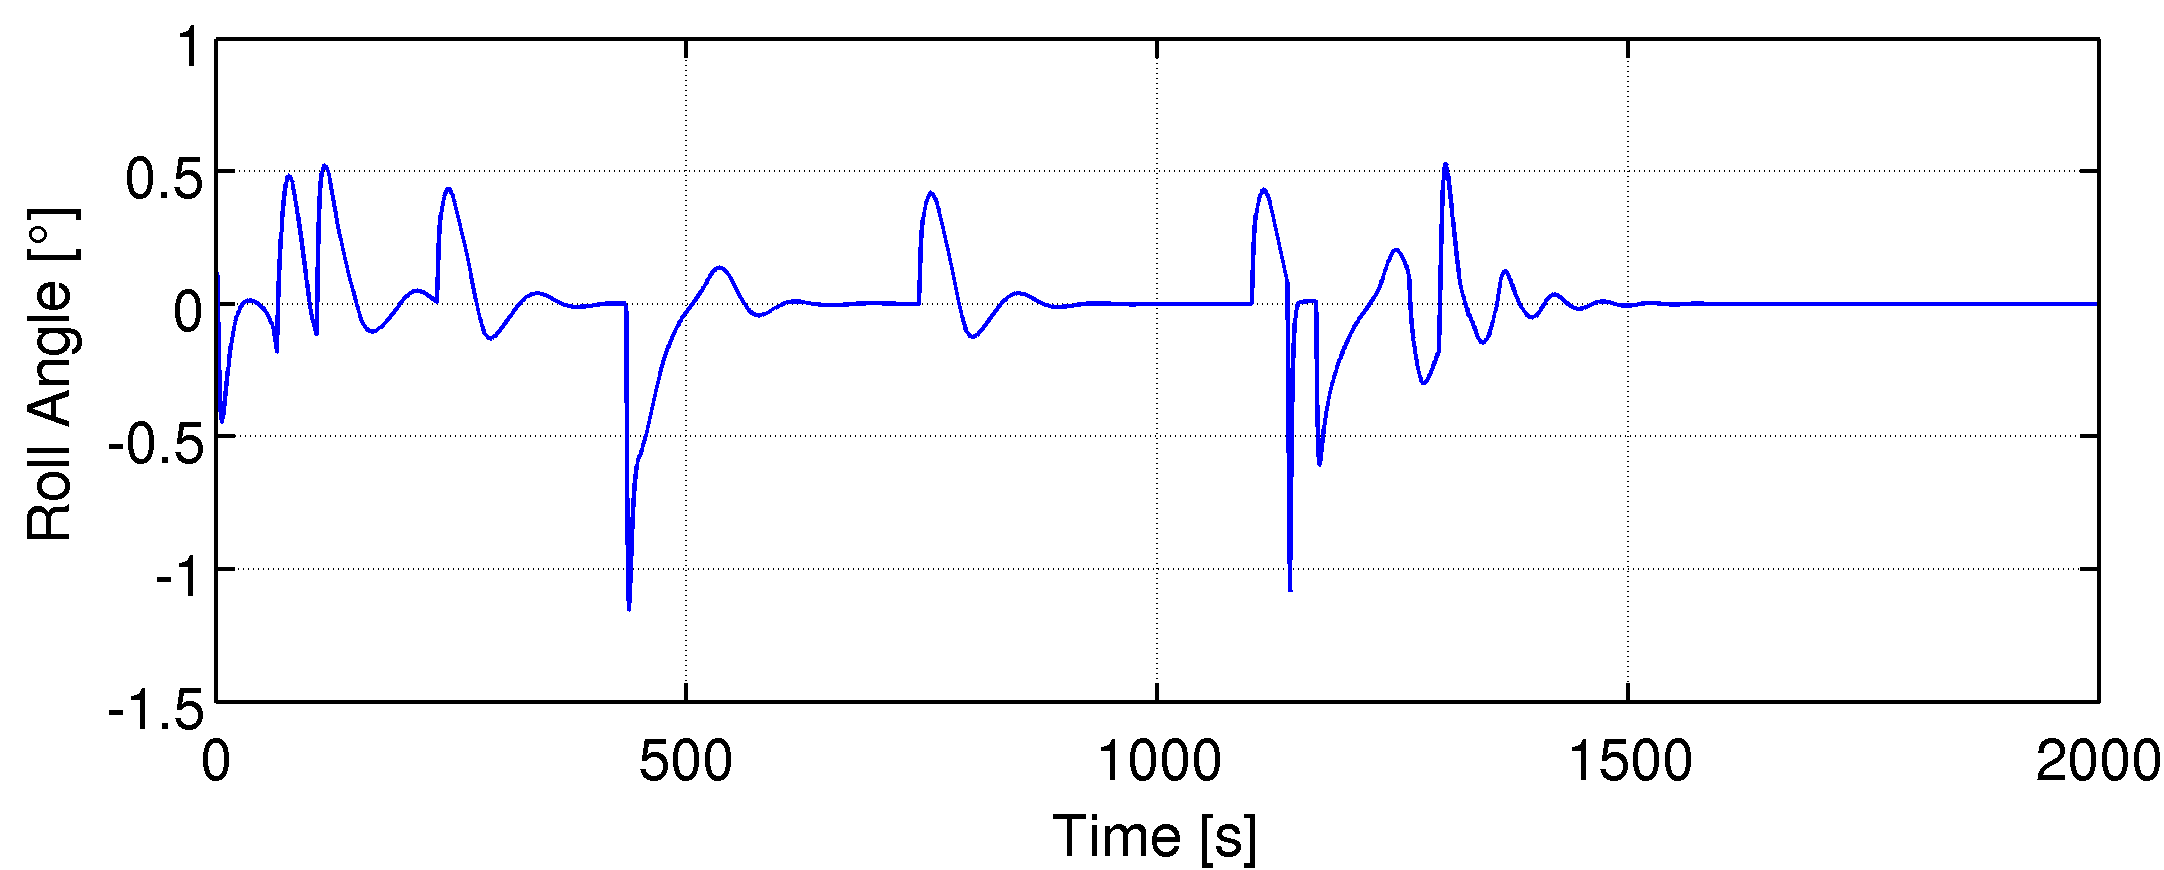
\includegraphics[width=0.7\textwidth]{pics/ch4_rollangle}}
		\subfigure[Yaw Moment]{
			\label{fig:ch4_yawmoment}
			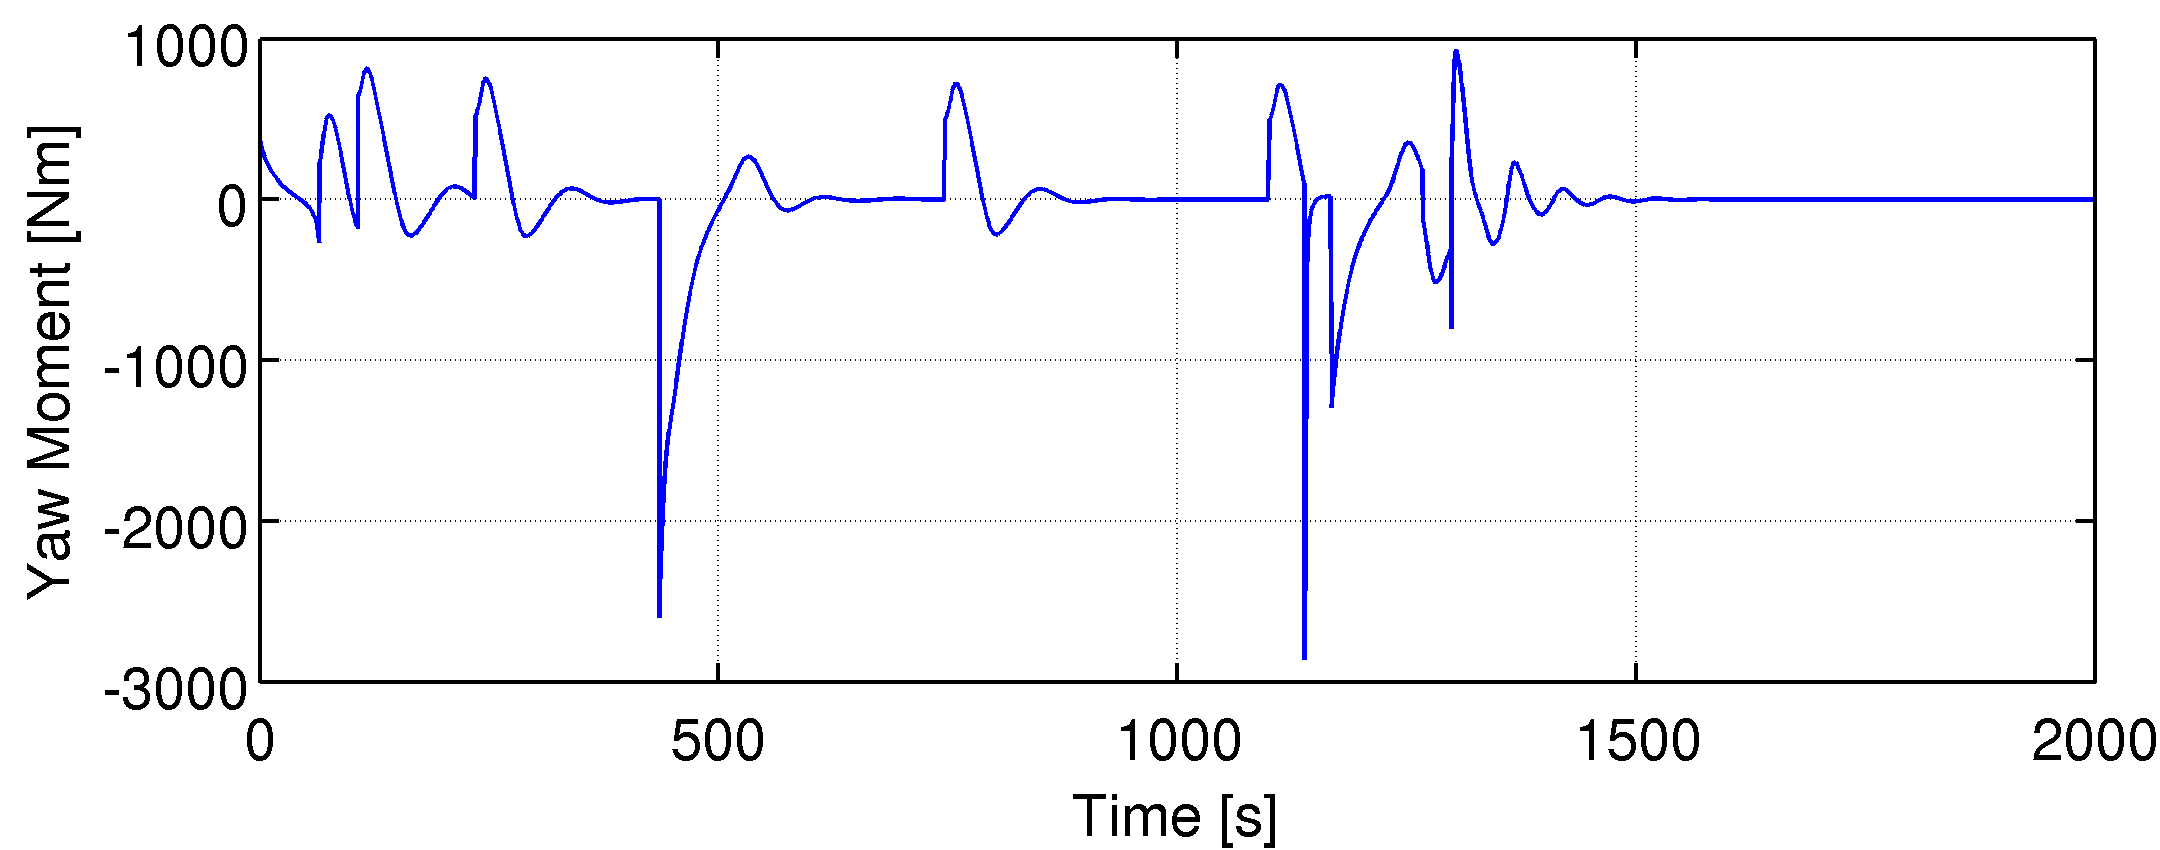
\includegraphics[width=0.7\textwidth]{pics/ch4_yawmoment}}
		\caption{Plots describing the close relation of yaw moment and roll angle}
		\label{fig:ch4_rollyawmoment}
	\end{figure}
	Figure~\ref{fig:ch4_rollyawmoment} shows the relation between commanded yaw moment and the roll angle.
	Clearly there are coupling effects which causes the roll angle to change a few degrees. The roll angle
	magnitude are about $1^\circ$ when the \textit{surge}-velocity are 1 m/s. The values of the
	\textit{roll} angle are doubled when the \textit{surge}-velocity are doubled. But the roll angle are not
	of great concern when carrying out this kind of inspection missions, as these simulations show.

	
	The main propeller gives a moment in roll. This moment are disregarded in the simulations, but might
	become important. The main propeller are described by the following relations
	\begin{equation}
		\begin{aligned}
			\tau_1 &= T_{nn} n^2 + T_{un} n u \\
			\tau_4 &= Q_{nn} n^2 + Q_{un} n u
		\end{aligned}
	\end{equation}
	where $n$ are the angular speed of the main propeller in revolutions per minute, and $u$ are again the
	surge velocity. The second terms in the equation above are terms describing loss-of-force due to
	forward speed. The moment in roll are actually countered by weighting the AUV down on one side so that when
	the it reaches cruise velocity the AUV have zero roll angle. \cite{Bjorn_gjelstad_talk}

	The \hugin AUV are designed to be asymptotically stable in roll, due to the centre of buoyancy (CB) are
	located not exactly in the centre of
	gravity (CG). The AUV would not need roll stabilisation because it in fact shows to be very stable in roll.


\section{Energy Consumption}
	The energy consumption of an AUV are of extreme importance. When a customer are buying this type of
	vessel, one of the criteria are operation time. For an AUV which are untethered and have limited power 
	supply the operation time might vary greatly due to installed sensors and operating conditions.

	The standard sensor suite on the \hugin AUV are a Side Scan Sonar, Doppler Velocity Log, Depth meter,
	Multibeam Echosounder, and the INS navigation system. The operation time would be around 10-20 hours,
	dependent on velocity and sensor use. The objective of the guidance system after the inspection
	part, is to maximise the operation time. This can be done in numerous ways, and should be a part of the
	design procedure when designing the guidance system for the real thing.

	The actuator set-up of \hugin  are 4 rudders, one main propeller and 4 thrusters. This renders
	the AUV controllable in 5 DOFs. The thrusters demand more power than the main propeller
	and rudders. Since this report considered the most energy efficient control, the thrusters have been disregarded
	throughout this report, but they will be of use if more advanced features should be implemented in the guidance
	system, such as docking of the AUV to an underwater charging station.

	The most energy efficient way of guiding an AUV is to use its main propeller and rudders. But there
	might be different ways of optimising the power consumption with regard to how the AUV are searching
	for, and tracking the pipeline. The moment produced by, for instance the vertical rudders, are 
	proportional to the \textit{surge-}velocity squared.
		\begin{equation}
			\tau_6 = Y_{u\psi} \delta u^2
		\end{equation}
	where $\delta$ are the angle of the rudder, and $Y_{u \psi}$ are some constant describing the rudder
	areal. This means that the effect of the rudders are greatly dependent on the forward speed. This is
	not taken into account in the designed controller and should be compensated for in a more advanced
	controller. This produces problems when the AUV are moving at greater velocities. Since the
	controller only	outputs moments which are not dependent on velocity, the AUV will have less maneuverability at
	higher speeds. This causes the proposed guidance scheme to fail at surge speeds higher than $1$ m/s if the
	controller are not re-tuned.

	The energy consumption are very dependent on how the AUV moves. If it is taking unnecessary turns the
	movement pattern are not optimal. If the forward speed are taken constant, the power consumption will
	decrease along with the AUV time-of-flight. In this sense the shortest distance travelled is the most
	optimal	movement pattern. This motivates the designer to make the guidance system to always calculate
	the shortest 
	path to the goal, if the environment allows it. This opens for a more advanced mode of the tracking
	system, where the constraint that the AUV should strictly follow the pipeline, are relaxed. If sensors
	like Sidescan Sonar or other sensors with longer range than a video camera are included, these can 
	be used to give good data about the pipeline even if it
	is not in the camera field of view. The relaxation in the tracking constraints might allow the AUV to
	move more efficient in terms of energy consumption.
	
	\cite{fuel_optimal_control} proposes an optimal guidance scheme. Using the
	fuel consumption as a performance index and optimise with regard to the ocean currents in the area of
	interest. It requires knowledge of the currents in the area \'a priori, and utilises this to calculate
	the optimal trajectory from one point to the next. This gives good theoretical results, but the
	downside
	is that knowledge about the current forces in an area are rarely known, and if they are known they are
	probably not very exact. But this scheme might help to save energy, but are only applicable to a
	pipeline inspection mission when the AUV are moving to, or from the pipeline.
	
	Either way, it is important to chose the right way to go when you have limited power capability. This
	motivates the use of more sensors, to increase the chances of not giving bad and erroneous sensor data
	to the guidance system. The guidance system needs to be robust and take the right decision. To
	maximise the operation time, it can not afford to take wrong decisions. This is almost impossible to
	achieve and can only be done through extensive testing of the complete system.

	The velocity of the AUV are of great importance. Since the AUV will experience drag effects by the
	water, and those effects are proportional to the velocity, the operation time will be greatly
	dependant on the speed. The equation below describes the relation between speed and range \cite{range}
	\begin{equation}
		R = \frac{E}{K_D} u^{-2}
	\end{equation}
	where $R$ is the range the AUV can travel in meters, $E$ is the available energy in Joules, $K_D$ is
	the efficient drag coefficient in W m$^3$/s$^3$ and $u$ is the velocity in m/s. This shows that the
	guidance system should control the speed in preference with what is most important. This
	relation are good for torpedo shaped AUVs such as \hugin, but it only apply when the AUV are moving
	at cruise speed, and not when it are using its thrusters.


\section{Optimal Search Pattern}
	As discussed above, the need for efficient search pattern are crucial to maximising the operation
	time. Search patterns might vary form case to case. The search patten should be dependent on how well
	the mission area are known and how sure one can be about the \'a priori data about the pipeline, sea
	bottom obstacles and other features. Are there obstacles in the area which might be used for
	position identification and navigation? Or are there obstacles in the area that the AUV should avoid
	completely, such as mines? This is information which are crucial when customising the search patterns.

	In general the more you know about the mission area, the better can you prepare the AUV for the
	mission. If there are known features on the sea bottom, those can be used as reference marks and
	navigation of the AUV. This allows for more customised search pattern which suit the mission area. 

\section{Validation of the Results}
	The analysis done in this report are meant to be a pre-study of the problems associated with this
	complex pipeline inspection problem. Most of the topics covered in this report need more study to get
	valid results. But it shows some key features for a future design.

	The distance covered by piplines are large, but most of the pipelines laid today are flexible
	pipelines and can curve quite a lot, and the assumption about linear pipeline segments are a bit to
	simplifying. On the other hand it is not difficult to generalise the guidance system to consider
	nonlinear paths. 

	The visibility is another topic about this simulations. The visibility are quickly degrading as depth
	increases, and to get good pictures there must have a good source of light. The visibility at 300
	meters are probably less than 3 meters. This will greatly decrease the field of view of the camera.

	
